% \input{\pSections "sec-writ-large"}

\section{Writ Large}

%     %     %     %     %     %     %     %     %
\subsection{RCS Models}
\begin{frame}\frametitle{Goal: RCS Models in 3D}
	RCS models have been built in 2D. \\
	\bl{Extend to 3D} using the same MoM code. 
\end{frame}
		%
%     %     %     %     %     %     %     %     %
\subsection{Domains}

\begin{frame}{Fourier Domains in 1-, 2-, and 3D}
\begin{table}[htp]
	%\caption{default}
	\begin{center}
				%
		\begin{tabular}{ccc}
			        \raisebox{0.95cm}{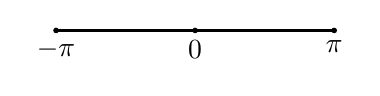
\begin{tikzpicture}[scale=0.75]
			        \begin{scope}[xshift=-5cm, yshift=0cm, scale=0.75]
            				\draw[thick] (-3.14,0) -- (3.14,0);
            				\foreach \x/\label in {-3.14/$-\pi$, 0/$0$, 3.14/$\pi$}
                				\draw[fill=black] (\x,0) circle (0.05) node[below] {\label};
        				\end{scope}
				\end{tikzpicture}} &
				%
			\includegraphics[ width = 3cm ]{ \pLocalGraphics/grid-2d.pdf } &
				%
			\includegraphics[ width = 3cm ]{ \pLocalGraphics/grid-3d.pdf } \\
				%
			$\theta \in \brac{-\pi, \pi}$ & $\theta \in \brac{-\pi, \pi}$ & $\theta \in \brac{-\pi, \pi}$ \\[5pt]
			& $r \in \brac{0,1}$ & $r \in \brac{0,1}$ \\[5pt]
			&& $\phi \in \brac{0,\pi}$
		\end{tabular}
	\end{center}
\label{tab:domains}
\end{table}%
\end{frame}

%     %     %     %     %     %     %     %     %
\subsection{Approximation}
\begin{frame}{Fourier and Extensions to 2- and 3-D}
    \centering
    $\fourier$
    \vspace{1em}
    \textit{From periodic functions in 1D to radial and angular decompositions in 2D and 3D.}
\end{frame}
	
\begin{frame}{Why We Love Fourier for Smooth Functions}
    \bl{Smooth Functions, Beautiful Representations}
    \begin{itemize}
        \item \bl{Weierstrass Approximation Theorem:} 
        Any continuous function on \([a, b]\) can be uniformly approximated by polynomials. Fourier provides a similar approximation, using trigonometric bases instead of polynomials.
        
        \item \bl{Riesz-Fischer Theorem:} 
        Hunting license - Fourier coefficients \((a_n, b_n)\) $\in$ \(l^2\), guaranteeing convergence in the \(L^2\) sense.

        \item \bl{Uniform Convergence for Smooth Periodic Functions:} 
       Smooth (\(C^\infty\) or \(C^k\)) functions, Fourier series converge uniformly, ensuring no oscillatory artifacts (Gibbs phenomenon disappears).

        \item \bl{Orthogonality of Basis:} 
        Sines and cosines form an orthogonal basis in \(L^2\), enabling direct computation of coefficients via projection (Parseval's theorem quantifies energy distribution).

        \item \bl{Spectral Insights:} 
        Decomposes a function into frequency components, making smoothness and structure explicit. High smoothness = rapid Fourier coefficient decay.

        \item \bl{Compact Representation:} 
        Smooth functions require fewer terms for accurate approximation. High efficiency for practical computation and storage.

        \item \bl{Universality:} 
        Fourier's reach extends to PDEs, signal processing, and quantum mechanics. Smooth functions unlock the full power of these tools.
    \end{itemize}
    \vspace{1em}
    \bl{Takeaway:} Fourier connects smoothness, convergence, and representation, offering unmatched clarity and utility for periodic and localized phenomena.
\end{frame}

\begin{frame}{Fourier and Extensions to 2- and 3D}
    \centering
    \renewcommand{\arraystretch}{2.0}
    \setlength{\tabcolsep}{10pt} % Adjust column spacing
    
    \begin{tabular}{@{} l c @{}} % Align left and center without extra spacing
        \textcolor{blue}{\bl{1D:}} & 
        \( \displaystyle f(\theta) = \sum_{n=-\infty}^{\infty} a_{n} \fourier \) \\[1em]

        \textcolor{blue}{\bl{2D:}} & 
        \( \displaystyle f(r, \theta) = \sum_{n=0}^{\infty}\sum_{m=-n}^{n,2} a_{n}^{m} \mg{R_n^m(r)}  \fourier  \) \\[1em]

        \textcolor{blue}{\bl{3D:}} & 
        \( \displaystyle 
        f(r, \theta, \phi) = 
        \sum_{n=0}^{\infty}\sum_{m=-n}^{n} 
        a_{n}^{m} \mg{\sqrt{\frac{(2m+1)(m-n)!}{4\pi (m+n)!}} 
        P_l^m(\cos \theta)} \fourier 
        \)
    \end{tabular}
\end{frame}
	
\begin{frame}{Fourier and Extensions to 2- and 3D}
    \begin{itemize}
        \item \href{https://mathworld.wolfram.com/FourierSeries.html}{\bl{1D Fourier Series:}} Decomposes a periodic function \(f(\theta)\) into a sum of complex exponentials with coefficients \(a_n\) capturing the amplitudes of each frequency component.
        \item \href{https://mathworld.wolfram.com/ZernikePolynomial.html}{\bl{2D Fourier-Bessel:}} Extends Fourier analysis to two dimensions using radial functions \(R_n^m(r)\), often employed in circular domains or optical applications.
        \item \href{https://mathworld.wolfram.com/SphericalHarmonic.html}{\bl{3D Spherical Harmonics:}} Represents functions on a sphere using harmonics \(Y_l^m(\theta, \phi)\) and radial components \(R_l(r)\), crucial in fields like quantum mechanics and gravitational modeling.
    \end{itemize}
\end{frame}

\begin{frame}{Lowest Order Fourier Basic Functions}
    \centering
    \begin{columns}[c] % Center-align the columns
        % Left column: Even Parity
        \begin{column}{0.5\textwidth}
            \centering
            $f(-\theta) = f(\theta)$  \\[0.5em]
            \textbf{Even Parity} \\[0.5em]
            \includegraphics[width=0.8\linewidth]{\pLocalGraphics/fourier-cos.pdf}
        \end{column}

        % Right column: Odd Parity
        \begin{column}{0.5\textwidth}
            \centering
            $f(-\theta) = -f(\theta)$  \\[0.5em]
            \textbf{Odd Parity} \\[0.5em]
            \includegraphics[width=0.8\linewidth]{\pLocalGraphics/fourier-sin.pdf}
        \end{column}
    \end{columns}
\end{frame}

	\input{\pLocalSlides "slide-Lowest-Order-Zernikes"}


%     %     %     %     %     %     %     %     %
\subsection{Quality of Fit}

\endinput  %  ==  ==  ==  ==  ==  ==  ==  ==  ==
